\documentclass{article}
\usepackage{graphicx}
\usepackage{amsmath}
\usepackage{booktabs}
\usepackage{url}
\usepackage{float}
\usepackage{amsfonts}
\usepackage[utf8]{inputenc}
\usepackage{algorithm2e}
\usepackage{microtype}

\title{Progetto WATER 4.0}
\author{Giovanni Giuseppe Iacuzzo}
\date{17-07-2025}

\begin{document}
\sloppy
\maketitle

\section{Obiettivo Predittivo e Approccio Proposto}

L'obiettivo di questo studio è stimare in modo continuo l’ammontare complessivo di perdita idrica 
nella rete, inteso come somma delle dispersioni simulate lungo i diversi collegamenti di una rete idrica. 
L’analisi si basa su sequenze temporali multivariate acquisite da sensori distribuiti sul sistema idrico.

A differenza dei metodi tradizionali, che si concentrano prevalentemente sulla rilevazione binaria 
di anomalie~\cite{piller2020}, l’approccio proposto mira a quantificare l’intensità del fenomeno 
nel tempo. Questo tipo di previsione permette di intercettare variazioni graduali, fornendo una 
misura continua della severità delle perdite, utile per pianificare interventi mirati e 
tempestivi~\cite{candelieri2016, soldevila2016leak}.

Una stima continua di questo tipo abilita strategie di controllo predittivo, manutenzione proattiva 
e sistemi di allerta precoce, configurandosi come uno strumento di supporto decisionale avanzato 
per i gestori della rete. Inoltre, l’adozione di modelli di deep learning consente di 
affrontare efficacemente la complessità e la non linearità dei dati, garantendo una buona 
capacità di generalizzazione anche in presenza di variabilità stagionali o dinamiche anomale~\cite{bao2019}.

\section{Definizione del Problema}

Negli ultimi anni, algoritmi ispirati all’intelligenza collettiva, come il \textit{Particle Swarm Optimization} 
(PSO), si sono dimostrati efficaci nell'affrontare problemi di ottimizzazione complessi~\cite{kennedy1995particle, 
eberhart2001pso}. 

In questo studio, proponiamo un approccio distribuito basato su una variante parallela e 
continua del PSO, nota come Continuous PSO (CPSO). L’idea centrale è sfruttare il parallelismo 
intrinseco dell’algoritmo swarm-based distribuendo il carico computazionale su più core CPU. A tale 
scopo, adottiamo il paradigma del \textit{modello a isole} (\textit{Island Model})~\cite{cantupaz1998survey, 
tomassini2005spatially}, che introduce un meccanismo di cooperazione asincrona tra sottopopolazioni 
evolutive.

In questo contesto, lo swarm viene suddiviso in sottoinsiemi indipendenti (le “isole”), ciascuno dei 
quali evolve in parallelo secondo le regole canoniche del CPSO~\cite{Ricciardello2020}. A intervalli 
regolari, le isole effettuano una sincronizzazione parziale mediante scambio delle migliori soluzioni 
globali. Questo meccanismo favorisce la diversità topologica e riduce il rischio di convergenza prematura, 
problematica frequente negli algoritmi swarm-based applicati a spazi ad alta dimensionalità~\cite{omran2005dynamic}.

Il \textit{modello a isole} costituisce un’estensione naturale degli approcci evolutivi e swarm-based, in cui 
la popolazione globale è suddivisa in sottopopolazioni autonome che evolvono in parallelo. La comunicazione 
tra isole avviene tramite \textit{migrazione} periodica delle migliori soluzioni, bilanciando l'esplorazione 
distribuita con la cooperazione tra i processi~\cite{tomassini2005spatially, cantupaz1998survey}.

La formulazione classica del CPSO~\cite{Ricciardello2020} descrive l’evoluzione delle particelle come la 
soluzione di un problema di Cauchy a coefficienti costanti a tratti. Tale approccio si è dimostrato 
superiore rispetto al PSO standard in termini di probabilità di successo e rapidità di convergenza, in 
particolare in problemi ad alta dimensionalità e con funzioni obiettivo non lineari e multimodali.

Per estendere questi vantaggi anche in ambienti paralleli, proponiamo un’implementazione distribuita del 
CPSO secondo il paradigma del \textit{modello a isole}, denominata \textit{Island-CPSO}. L’algoritmo 
suddivide lo swarm in sottopopolazioni indipendenti che evolvono in parallelo e si sincronizzano 
periodicamente attraverso meccanismi di migrazione.

\section{Dataset Utilizzato}

Il presente studio si avvale del dataset rilasciato nell'ambito della competizione internazionale 
BattLeDIM 2020 (Battle of the Leakage Detection and Isolation Methods) ~\cite{battle2020}, finalizzata allo 
sviluppo di metodologie avanzate per la rilevazione e la localizzazione di perdite nei sistemi di distribuzione 
idrica. I dati utilizzati derivano da simulazioni sul modello \emph{L-Town}, una rete idrica virtuale dettagliata, 
ispirata a condizioni operative realistiche.

\begin{figure}[htbp]
    \centering
    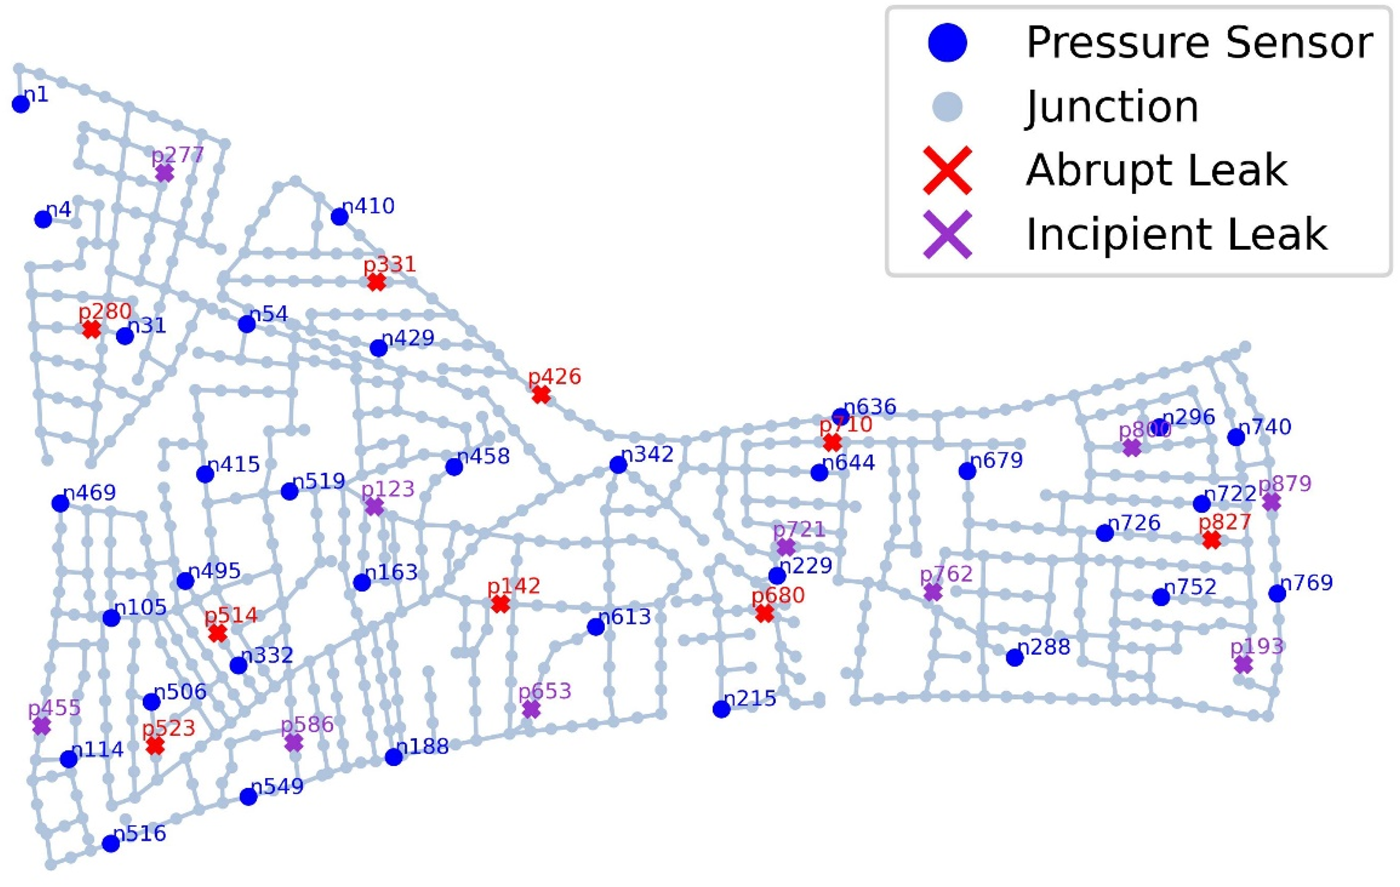
\includegraphics[width=0.6\textwidth]{img/struttura della rete.png}
    \caption{Struttura della rete idrica considerata.}
    \label{fig:network_structure}
\end{figure}

Il dataset comprende misurazioni con cadenza di 5 minuti relative a due anni consecutivi (2018--2019). 
In questa ricerca ci si è concentrati esclusivamente sull'anno 2018, utilizzando le seguenti tipologie 
di variabili:

\begin{itemize}
    \item \textbf{Domande (Demands)}: flussi di consumo registrati da 82 dispositivi di lettura automatica.
    \item \textbf{Flussi (Flows)}: portate in ingresso/uscita rilevate da 3 sensori distribuiti.
    \item \textbf{Livelli (Levels)}: livelli dell’acqua in un serbatoio, espressi in metri.
    \item \textbf{Pressioni (Pressures)}: misure in metri presso 33 punti della rete.
    \item \textbf{Perdite (Leakages)}: tassi di perdita (in m$^3$/h) simulati su specifici collegamenti, utilizzati come variabile target.
\end{itemize}

Tutte le serie temporali sono fornite in formato \texttt{CSV}, allineate temporalmente
tramite timestamp. I dati sono stati integrati e preprocessati per formare una matrice 
temporale multivariata coerente, normalizzata tramite \texttt{StandardScaler}, e segmentata 
in finestre mobili di lunghezza fissa (\texttt{seq\_len}). A ciascuna finestra di input è 
associato, come target, il valore della perdita totale nel timestamp successivo.

\section{Architettura del Modello LSTM}

L’analisi di dati temporali provenienti da una rete idrica, raccolti a intervalli regolari, 
richiede modelli in grado di catturare le dipendenze sequenziali tra le osservazioni. 
Le \emph{reti neurali ricorrenti} (Recurrent Neural Networks, RNN) rispondono a questa 
esigenza grazie alla loro struttura con memoria interna, che consente di apprendere relazioni 
temporali tra gli input successivi~\cite{elman1990finding}. Tuttavia, le RNN tradizionali 
presentano limiti nella gestione delle dipendenze a lungo termine, principalmente a causa di 
problemi di vanishing e exploding gradient durante l'addestramento~\cite{bengio1994learning}.

Per superare tali limitazioni, viene adottata una variante delle RNN nota come 
\emph{Long Short-Term Memory} (LSTM), introdotta da Hochreiter e 
Schmidhuber~\cite{hochreiter1997long}. Le reti LSTM sono progettate per mantenere informazioni 
rilevanti anche a distanza di molti passi temporali, grazie a un meccanismo interno di memoria 
controllata. Questo meccanismo è regolato da tre componenti principali, detti \emph{gate}, 
che modulano dinamicamente l’ingresso, la conservazione e l’uscita delle informazioni.

Nel presente lavoro, si utilizza un modello LSTM per prevedere la quantità attesa di perdita 
idrica al passo temporale successivo, sulla base di una sequenza storica di osservazioni. 
Ogni input al modello è rappresentato da una sequenza temporale multivariata di dimensione 
$(T, F)$, dove $T$ indica la lunghezza della finestra temporale e $F$ il numero di feature 
disponibili. L’output è un singolo valore scalare $\hat{y}_{T+1}$, che rappresenta la stima 
della perdita al tempo $T+1$.

La calibrazione automatica del modello LSTM è effettuata tramite la strategia 
\emph{Island-CPSO}. La funzione obiettivo da minimizzare è definita come la perdita sul 
validation set per una data configurazione di iperparametri, tra cui: numero di layer, dimensione 
dello stato nascosto, tasso di dropout e learning rate.

Formalmente, il problema di ottimizzazione si esprime come:

\begin{equation}
\min_{\theta \in \Theta} \mathcal{L}{val}(\mathcal{M}(\theta; \mathcal{D}{train}), \mathcal{D}_{val})
\end{equation}

dove $\theta \in \Theta \subset \mathbb{R}^d$ rappresenta il vettore degli iperparametri, $\mathcal{M}(\cdot)$ è il 
modello LSTM, $\mathcal{D}{train}$ e $\mathcal{D}{val}$ sono rispettivamente i dataset di addestramento e 
validazione, e $\mathcal{L}_{val}$ è la funzione di perdita calcolata sul validation set.

\subsection{Struttura della Cella LSTM}

Ogni cella LSTM riceve in input lo stato precedente e il dato corrente, e aggiorna selettivamente 
la propria memoria, questo è possibile grazie all’impiego di tre componenti fondamentali, chiamati 
\textit{gate}, che regolano dinamicamente il flusso delle informazioni. In particolare, il forget 
gate determina quali contenuti della memoria passata devono essere eliminati; l’input gate stabilisce 
quali nuove informazioni devono essere integrate; infine, l’output gate seleziona cosa dev’essere 
restituito come risultato del passo corrente.

Tutte queste operazioni si basano su trasformazioni affini dei dati di input e dell’output precedente, 
seguite da funzioni di attivazione non lineari, generalmente la sigmoide o la tangente iperbolica. 
Analizziamo ora in dettaglio il comportamento interno della cella al tempo $t$.

Il primo passo consiste nel calcolo del forget gate $f_t$, che ha il compito di decidere quali parti 
dello stato di memoria precedente, $c_{t-1}$, devono essere mantenute:
\begin{equation}
f_t = \sigma(W_f x_t + U_f h_{t-1} + b_f)
\end{equation}
Qui, $x_t$ rappresenta l’input corrente, $h_{t-1}$ l’output della cella al passo precedente, e i 
parametri $W_f$, $U_f$ e $b_f$ sono i pesi e il bias del gate. La funzione sigmoide $\sigma$ restituisce 
valori compresi tra 0 e 1, che agiscono da fattori di selezione sulle componenti della memoria.

Segue il calcolo dell’input gate $i_t$, che serve a valutare quante delle nuove informazioni, elaborate 
dall’input corrente, devono essere effettivamente acquisite:
\begin{equation}
i_t = \sigma(W_i x_t + U_i h_{t-1} + b_i)
\end{equation}

Contemporaneamente, viene generato un candidato $\tilde{c}_t$ per il nuovo contenuto da inserire nello 
stato interno, applicando una tangente iperbolica a una trasformazione lineare dell’input e dell’output 
precedente:
\begin{equation}
\tilde{c}_t = \tanh(W_c x_t + U_c h_{t-1} + b_c)
\end{equation}

A questo punto, lo stato interno della cella viene aggiornato combinando l’informazione precedente e 
quella appena calcolata. Il forget gate determina quanta memoria passata viene trattenuta, mentre 
l’input gate stabilisce quanto del nuovo contenuto deve essere integrato:
\begin{equation}
c_t = f_t \odot c_{t-1} + i_t \odot \tilde{c}_t
\end{equation}
dove $\odot$ rappresenta il prodotto elemento per elemento.

Infine, l’output della cella viene calcolato in due passaggi. Prima si valuta l’output gate $o_t$, che 
decide quanta parte dello stato interno aggiornato deve essere resa disponibile all’esterno:
\begin{equation}
o_t = \sigma(W_o x_t + U_o h_{t-1} + b_o)
\end{equation}
Poi si applica una tangente iperbolica allo stato interno $c_t$ e lo si modula tramite $o_t$:
\begin{equation}
h_t = o_t \odot \tanh(c_t)
\end{equation}

Questa sequenza di operazioni consente alla cella LSTM di filtrare, aggiornare e trasmettere informazioni 
nel tempo in modo controllato e flessibile.

Per completezza, si riportano le principali notazioni utilizzate: $x_t \in \mathbb{R}^F$ è il vettore di 
input al tempo $t$, con $F$ caratteristiche; $h_{t-1}$ è l’output del passo precedente; $c_t$ rappresenta 
lo stato interno aggiornato; $\sigma$ e $\tanh$ indicano rispettivamente le funzioni di attivazione 
sigmoide e tangente iperbolica; infine, $\odot$ denota il prodotto elemento per elemento.

Una rappresentazione grafica del funzionamento della cella LSTM è riportata in Figura~\ref{fig:lstm_cell}, 
utile per visualizzare il flusso interno delle informazioni.

\begin{figure}[htbp]
    \centering
    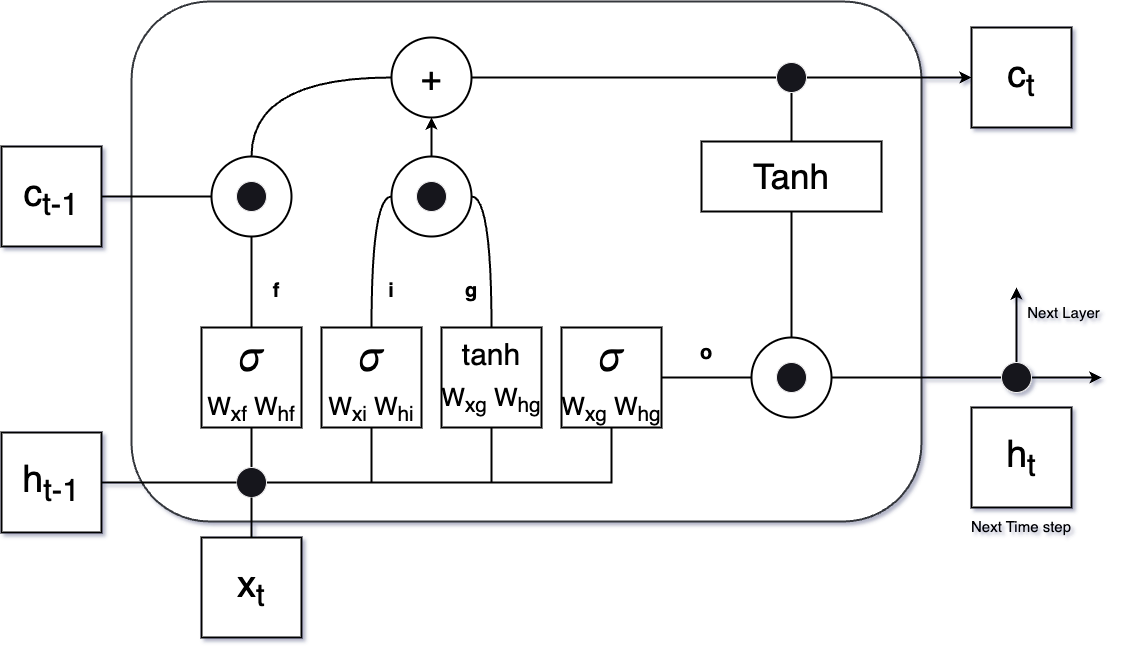
\includegraphics[width=0.6\textwidth]{img/LSTM.png}
    \caption{Struttura interna di una cella LSTM, con evidenza dei tre gate principali e dello stato di memoria.}
    \label{fig:lstm_cell}
\end{figure}

L’architettura del modello è strutturata come segue:

\begin{itemize}
    \item \textbf{Primo strato LSTM}: elabora la sequenza temporale in input producendo rappresentazioni latenti. Il numero di unità è un iperparametro ottimizzato.
    \item \textbf{Secondo strato LSTM}: riceve l'output del primo strato, sintetizzando ulteriormente le informazioni nel tempo. È configurato con \verb|return_sequences=False|.
    \item \textbf{Dropout}: applicato per la regolarizzazione, con tasso anch'esso ottimizzato.
    \item \textbf{Strato denso finale}: un neurone completamente connesso con attivazione lineare che restituisce il valore continuo della perdita.
\end{itemize}

Il modello è addestrato tramite la minimizzazione della \textit{Mean Squared Error (MSE)} tra la 
previsione $\hat{y}_{T+1}$ e il valore reale $y_{T+1}$, secondo l’obiettivo:

\begin{equation}
\mathcal{L} = \frac{1}{N} \sum_{i=1}^N \left( \hat{y}_{i} - y_{i} \right)^2
\end{equation}

dove $N$ è il numero totale di esempi nella finestra mobile di addestramento.

\section{Modello Island}

Il modello a isole si fonda su una suddivisione della popolazione globale $\mathcal{P}$ in $K$ sottopopolazioni 
disgiunte (isole), come proposto in \cite{alba2002parallelism, tomassini2005spatially}:
\begin{equation}
\mathcal{P} = \bigcup_{k=1}^K \mathcal{P}_k \quad \text{con} \quad \mathcal{P}_i \cap \mathcal{P}_j = \emptyset \quad \forall i \neq j
\end{equation}
dove $\mathcal{P}_k = \{x_1^{(k)}, x_2^{(k)}, \dots, x_{n_k}^{(k)}\}$ rappresenta la popolazione dell'isola $k$ con $n_k$ individui/particelle.

Ogni individuo $x_i^{(k)} \in \mathbb{R}^d$ rappresenta una possibile soluzione nel dominio degli 
iperparametri $\Theta \subseteq \mathbb{R}^d$, e viene valutato da una funzione obiettivo locale, 
coerente con l'approccio seguito nei modelli di ottimizzazione distribuita di iperparametri \cite{li2019openbox}:
\begin{equation}
f^{(k)} : \Theta \to \mathbb{R}, \quad f^{(k)}(x) = \mathcal{L}_{val}(\mathcal{M}(x; \mathcal{D}_{train}^{(k)}), \mathcal{D}_{val}^{(k)})
\end{equation}

La dinamica evolutiva in ciascuna isola segue un algoritmo base $A$, che viene applicato localmente 
secondo una funzione di aggiornamento $\phi_A$, come descritto in \cite{kennedy1995particle, engelbrecht2007computational}:
\begin{equation}
\mathcal{P}_k^{(t+1)} = \phi_A(\mathcal{P}_k^{(t)})
\end{equation}

Il concetto di migrazione regolare è una delle componenti chiave del modello a isole e viene 
generalmente attivato ogni $T_m \in \mathbb{N}$ iterazioni \cite{tomassini2005spatially}. 
Le connessioni tra isole possono essere descritte da un grafo diretto $G = (V, E)$, seguendo una 
topologia predefinita (completa, anello, bidirezionale, ecc.), secondo le analisi in \cite{cantupaz1998survey}.

La funzione di migrazione $\mu$ agisce come segue:

\begin{equation}
\mu: \mathcal{P}_i \times \mathcal{P}_j \rightarrow \mathcal{P}_j, \quad \mu(S_i, \mathcal{P}_j) = \mathcal{P}_j'
\end{equation}

dove $S_i \subseteq \mathcal{P}_i$ è un sottoinsieme degli individui migliori (secondo $f^{(i)}$), e i loro 
corrispettivi rimpiazzano i peggiori individui in $\mathcal{P}_j$ come discusso in \cite{alba2002parallelism}.

Il processo iterativo globale può quindi essere riassunto come:

\begin{enumerate}
    \item Per ogni isola $k$, applicare $\phi_A$ per $T_m$ iterazioni.
    \item Eseguire $\mu$ secondo $G$ e aggiornare le popolazioni locali.
    \item Ripetere fino a convergenza o budget massimo di iterazioni.
\end{enumerate}

\subsection{Parallelizzazione e Complessità}

L'analisi computazionale del modello a isole mostra un'efficienza elevata grazie alla decomposizione 
naturale del problema in sottoprocessi paralleli \cite{alba2005parallel}. Sia $C_{eval}$ il costo medio 
di valutazione della funzione obiettivo. In un sistema seriale il costo totale è:
\begin{equation}
\mathcal{C}_{serial} = \mathcal{O}(N \cdot T \cdot C_{eval})
\end{equation}

Nel contesto distribuito con $K$ isole di dimensioni simili ($n_k \approx N/K$), e con una migrazione 
sincronizzata ogni $T_m$ iterazioni, il costo teorico diventa:
\begin{equation}
\mathcal{C}_{parallel} = \mathcal{O}\left(\frac{N \cdot T \cdot C_{eval}}{K} + \frac{T}{T_m} \cdot C_{migrazione}\right)
\end{equation}

dove $C_{migrazione}$ è legato al costo della comunicazione e sincronizzazione, che può essere ridotto 
sfruttando modelli asincroni o a bassa frequenza di migrazione, come suggerito in \cite{cantupaz1998survey}.

Implementazioni efficienti sono state sviluppate usando paradigmi di memoria condivisa 
(es. \texttt{multiprocessing} in Python) o memoria distribuita (es. MPI), ottenendo significativi guadagni in 
termini di scalabilità \cite{alba2002parallelism, li2019openbox}.

\subsection{Benefici e Considerazioni}

Tra i principali vantaggi del modello a isole si possono evidenziare \cite{cantupaz1998survey, tomassini2005spatially}:

\begin{itemize}
    \item \textbf{Robustezza}: le isole esplorano indipendentemente lo spazio delle soluzioni, riducendo il rischio di convergenza prematura.
    \item \textbf{Parallelismo naturale}: la struttura a isole consente un'esecuzione intrinsecamente parallela.
    \item \textbf{Controllo della divergenza}: la migrazione regolare permette di riequilibrare sfruttamento ed esplorazione.
\end{itemize}

Tuttavia, la configurazione della topologia di comunicazione, della frequenza di migrazione $T_m$, e del 
numero di individui migranti è critica e deve essere ottimizzata empiricamente \cite{alba2002parallelism}.

L'implementazione parallela è ottenibile con paradigmi a memoria condivisa, come 
\texttt{multiprocessing} in Python o \texttt{OpenMP}/MPI in C++. Le strutture dati per la migrazione 
possono usare code FIFO, semafori o oggetti condivisi (\texttt{Manager.Queue} in Python). 
La sincronizzazione può essere sincrona (bloccante) o asincrona, a seconda dell’efficienza desiderata e 
del tipo di hardware.

\section{Algoritmo Island-CPSO}

Ogni isola è associata a un processo parallelo e contiene un sotto-swarm che evolve secondo la 
formulazione continua del CPSO. Ogni sotto-swarm segue localmente le equazioni differenziali descritte 
in \cite{Ricciardello2020}, ed effettua una valutazione autonoma della funzione obiettivo. Ad ogni 
intervallo di migrazione $T_m$, le isole si scambiano le migliori posizioni locali e aggiornano il 
proprio stato globale, favorendo così una convergenza cooperativa.

\subsection{Pseudo-codice}

Il seguente pseudo-codice descrive l’algoritmo \textit{Island-CPSO}:

\begin{algorithm}[H]
\caption{Island-CPSO}
\KwIn{Numero di isole $K$, dimensione swarm globale $N$, numero intervalli $T$, intervallo di migrazione $T_m$, funzione obiettivo $f$}
\KwOut{Miglior soluzione trovata $x^\ast$}

Suddividi lo swarm globale in $K$ isole: $\mathcal{P} = \bigcup_{k=1}^K \mathcal{P}_k$ con $|\mathcal{P}_k| = N/K$\\

\ForEach{isola $k \in \{1, \dots, K\}$ \textbf{in parallelo}}{
    Inizializza le posizioni $p^{(0)}_i$ e velocità $v^{(0)}_i$ delle particelle in $\mathcal{P}_k$\\
    Calcola $p_{\text{ib}}$ e $p_{\text{gb}}$ iniziali\\
    \For{$t = 1$ \KwTo $T$}{
        Calcola $f_k(t) = c_c r_1(t) \cdot p_{\text{ib}} + c_s r_2(t) \cdot p_{\text{gb}}$\\
        Calcola $\mu(t)$, $\zeta(t)$, $\omega(t)$ secondo \cite{Ricciardello2020}\\
        Risolvi il sistema ODE:
        \[
            \ddot{p}(t) + 2\zeta(t)\omega(t)\dot{p}(t) + \omega(t)^2 p(t) = f_k(t)
        \]
        Aggiorna $p_i(t), \dot{p}_i(t)$ per ogni particella\\
        Aggiorna $p_{\text{ib}}, p_{\text{gb}}$ locali
        \If{$t \bmod T_m = 0$}{
            Esegui \texttt{MIGRAZIONE}$(\mathcal{P}_k, \mathcal{P}_{\text{vicine}})$
        }
    }
}

Raccogli i migliori $p_{\text{gb}}^{(k)}$ da ogni isola e seleziona:
\[
x^\ast = \arg\min_{k} f(p_{\text{gb}}^{(k)})
\]

\textbf{return} $x^\ast$
\end{algorithm}

\subsection{Funzione di Migrazione}

La funzione \texttt{MIGRAZIONE} può essere definita secondo una topologia predefinita 
(es. anello, completamente connessa). Il meccanismo base consiste nel selezionare un sottoinsieme $S_k$ 
delle migliori particelle da $\mathcal{P}_k$ e sostituire le peggiori in $\mathcal{P}_j$, con $j \in \mathcal{N}(k)$.

\begin{algorithm}[H]
\caption{\texttt{MIGRAZIONE}$(\mathcal{P}_k, \mathcal{P}_{\text{vicine}})$}
\ForEach{$\mathcal{P}_j \in \mathcal{N}(k)$}{
    Seleziona $S_k \subseteq \mathcal{P}_k$ con le $m$ migliori particelle\\
    Sostituisci le $m$ peggiori in $\mathcal{P}_j$ con gli elementi di $S_k$\\
    Aggiorna $p_{\text{gb}}^{(j)}$ in base alla nuova popolazione
}
\end{algorithm}

\section{Risultati ottenuti}

In questa sezione si analizzano i risultati ottenuti con il modello LSTM 
ottimizzato mediante CPSO, con l’obiettivo di valutarne la capacità predittiva 
su dati non visti e la sua generale efficacia nel contesto del problema affrontato. 
Il modello è stato addestrato su una porzione dei dati e successivamente testato 
su un insieme separato.

Il processo di integrazione tra modello LSTM e ottimizzatore CPSO è illustrato nel diagramma di flusso 
in Figura~\ref{fig:cpso_flowchart}. Qui il CPSO genera nuove configurazioni, valuta 
le prestazioni del modello sul set di validazione e aggiorna la popolazione di particelle 
in base alla funzione obiettivo.

\begin{figure}[H]
\centering
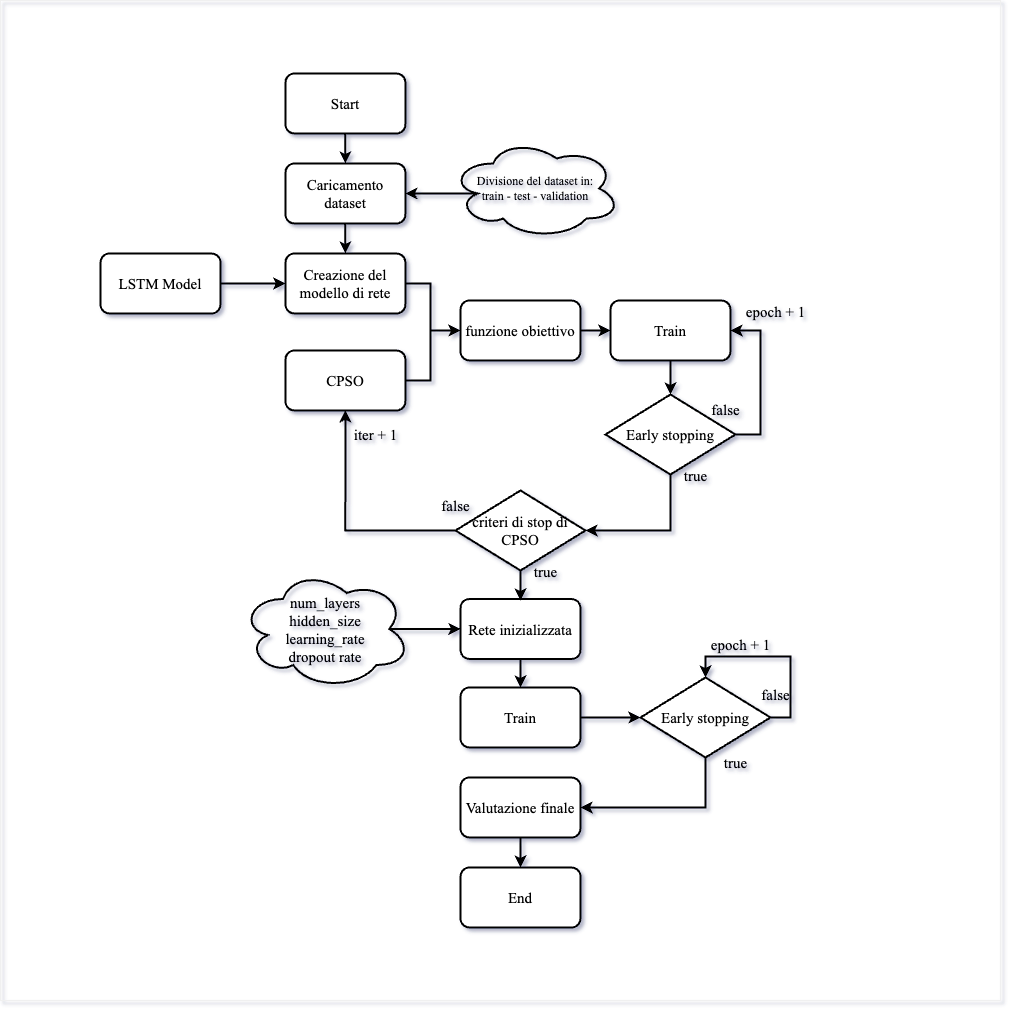
\includegraphics[width=0.8\textwidth]{img/LSTM-CPSO-MODEL.png}
\caption{Diagramma di flusso del processo di ottimizzazione del modello LSTM mediante CPSO.}
\label{fig:cpso_flowchart}
\end{figure}

Gli iperparametri ottimizzati dal CPSO includono:
\begin{itemize}
    \item \textbf{Numero di layer} LSTM ($\in [1, 5]$)
    \item \textbf{Dimensione dello stato nascosto} ($\in [16, 256]$)
    \item \textbf{Tasso di dropout} ($\in [0.0, 0.6]$)
    \item \textbf{Learning rate} ($\in [10^{-5}, 10^{-2}]$)
\end{itemize}

La funzione obiettivo utilizzata per guidare l’ottimizzazione è la minimizzazione della loss di validazione 
(MSE), calcolata su un set separato rispetto a quello di training.

\subsection{Analisi della convergenza e collaborazione tra isole}

La Figura~\ref{fig:convergenza_isole} mostra l'andamento delle curve di convergenza per ciascuna isola. 
Si osserva una progressiva riduzione della loss, con ogni isola che parte da condizioni iniziali differenti 
ma tende a convergere verso un minimo comune. Ciò è reso possibile dalla strategia di migrazione, che 
permette lo scambio delle migliori soluzioni tra le popolazioni.

\begin{figure}[H]
    \centering
    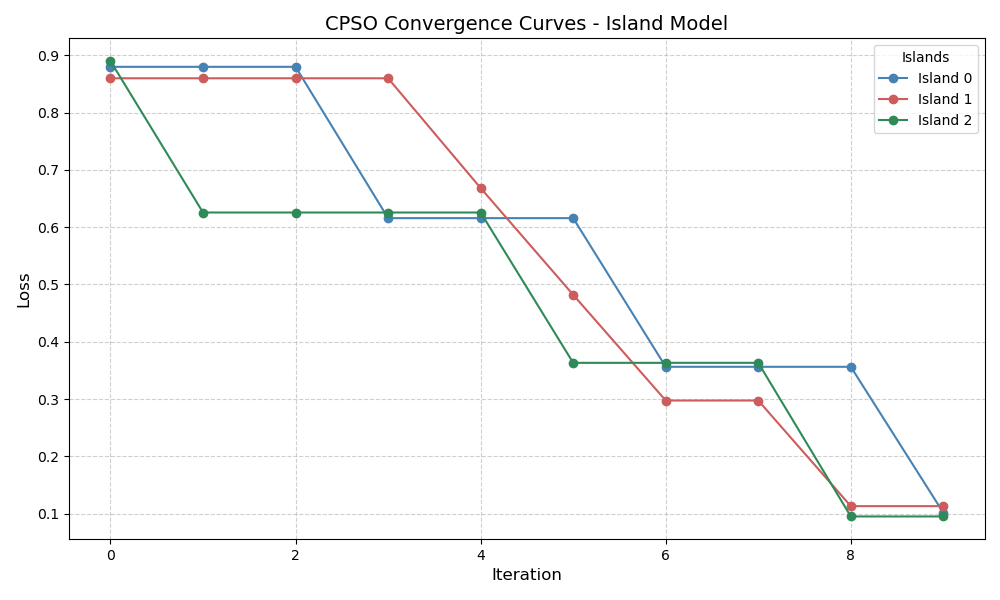
\includegraphics[width=0.9\textwidth]{img/CPSO Convergence Curves - Island Mode.png}
    \caption{Curve di convergenza delle singole isole durante l’ottimizzazione CPSO.}
    \label{fig:convergenza_isole}
\end{figure}

La Figura~\ref{fig:global_cost} rappresenta invece l’evoluzione del miglior costo globale dopo ogni migrazione. 
Questo grafico fornisce una visione complessiva della capacità dell’algoritmo di migliorare iterativamente la 
soluzione globale grazie alla cooperazione tra isole.

\begin{figure}[H]
    \centering
    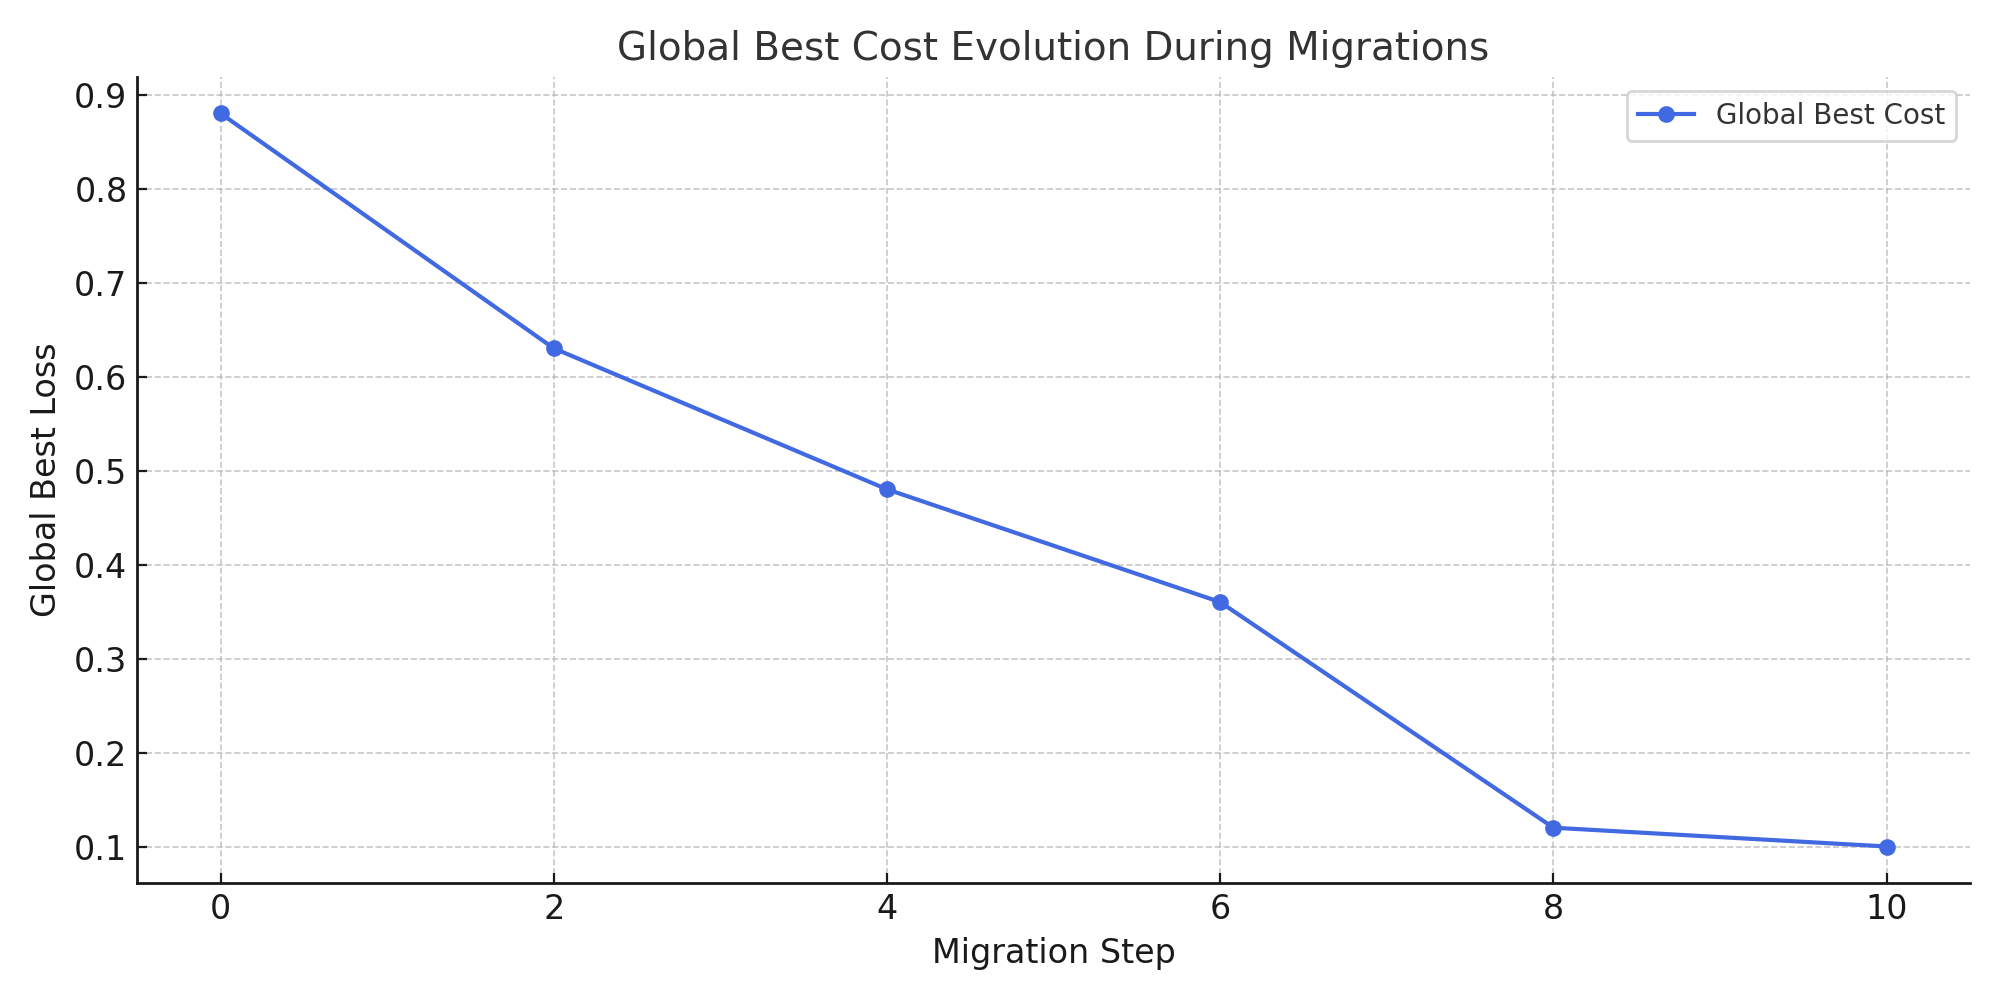
\includegraphics[width=0.75\textwidth]{img/global_best_cost_per_migration.png}
    \caption{Andamento del miglior costo globale al termine di ciascuna migrazione.}
    \label{fig:global_cost}
\end{figure}

Infine, la Figura~\ref{fig:final_costs_hist} mostra la distribuzione dei costi finali ottenuti da ogni isola al 
termine dell’ultima migrazione. Questo istogramma è utile per valutare se le isole convergono in modo coerente o 
se esistono isole che faticano a seguire il progresso globale. Una distribuzione compatta, come quella osservata, 
è indicativa di una buona sincronizzazione e collaborazione.

\begin{figure}[H]
    \centering
    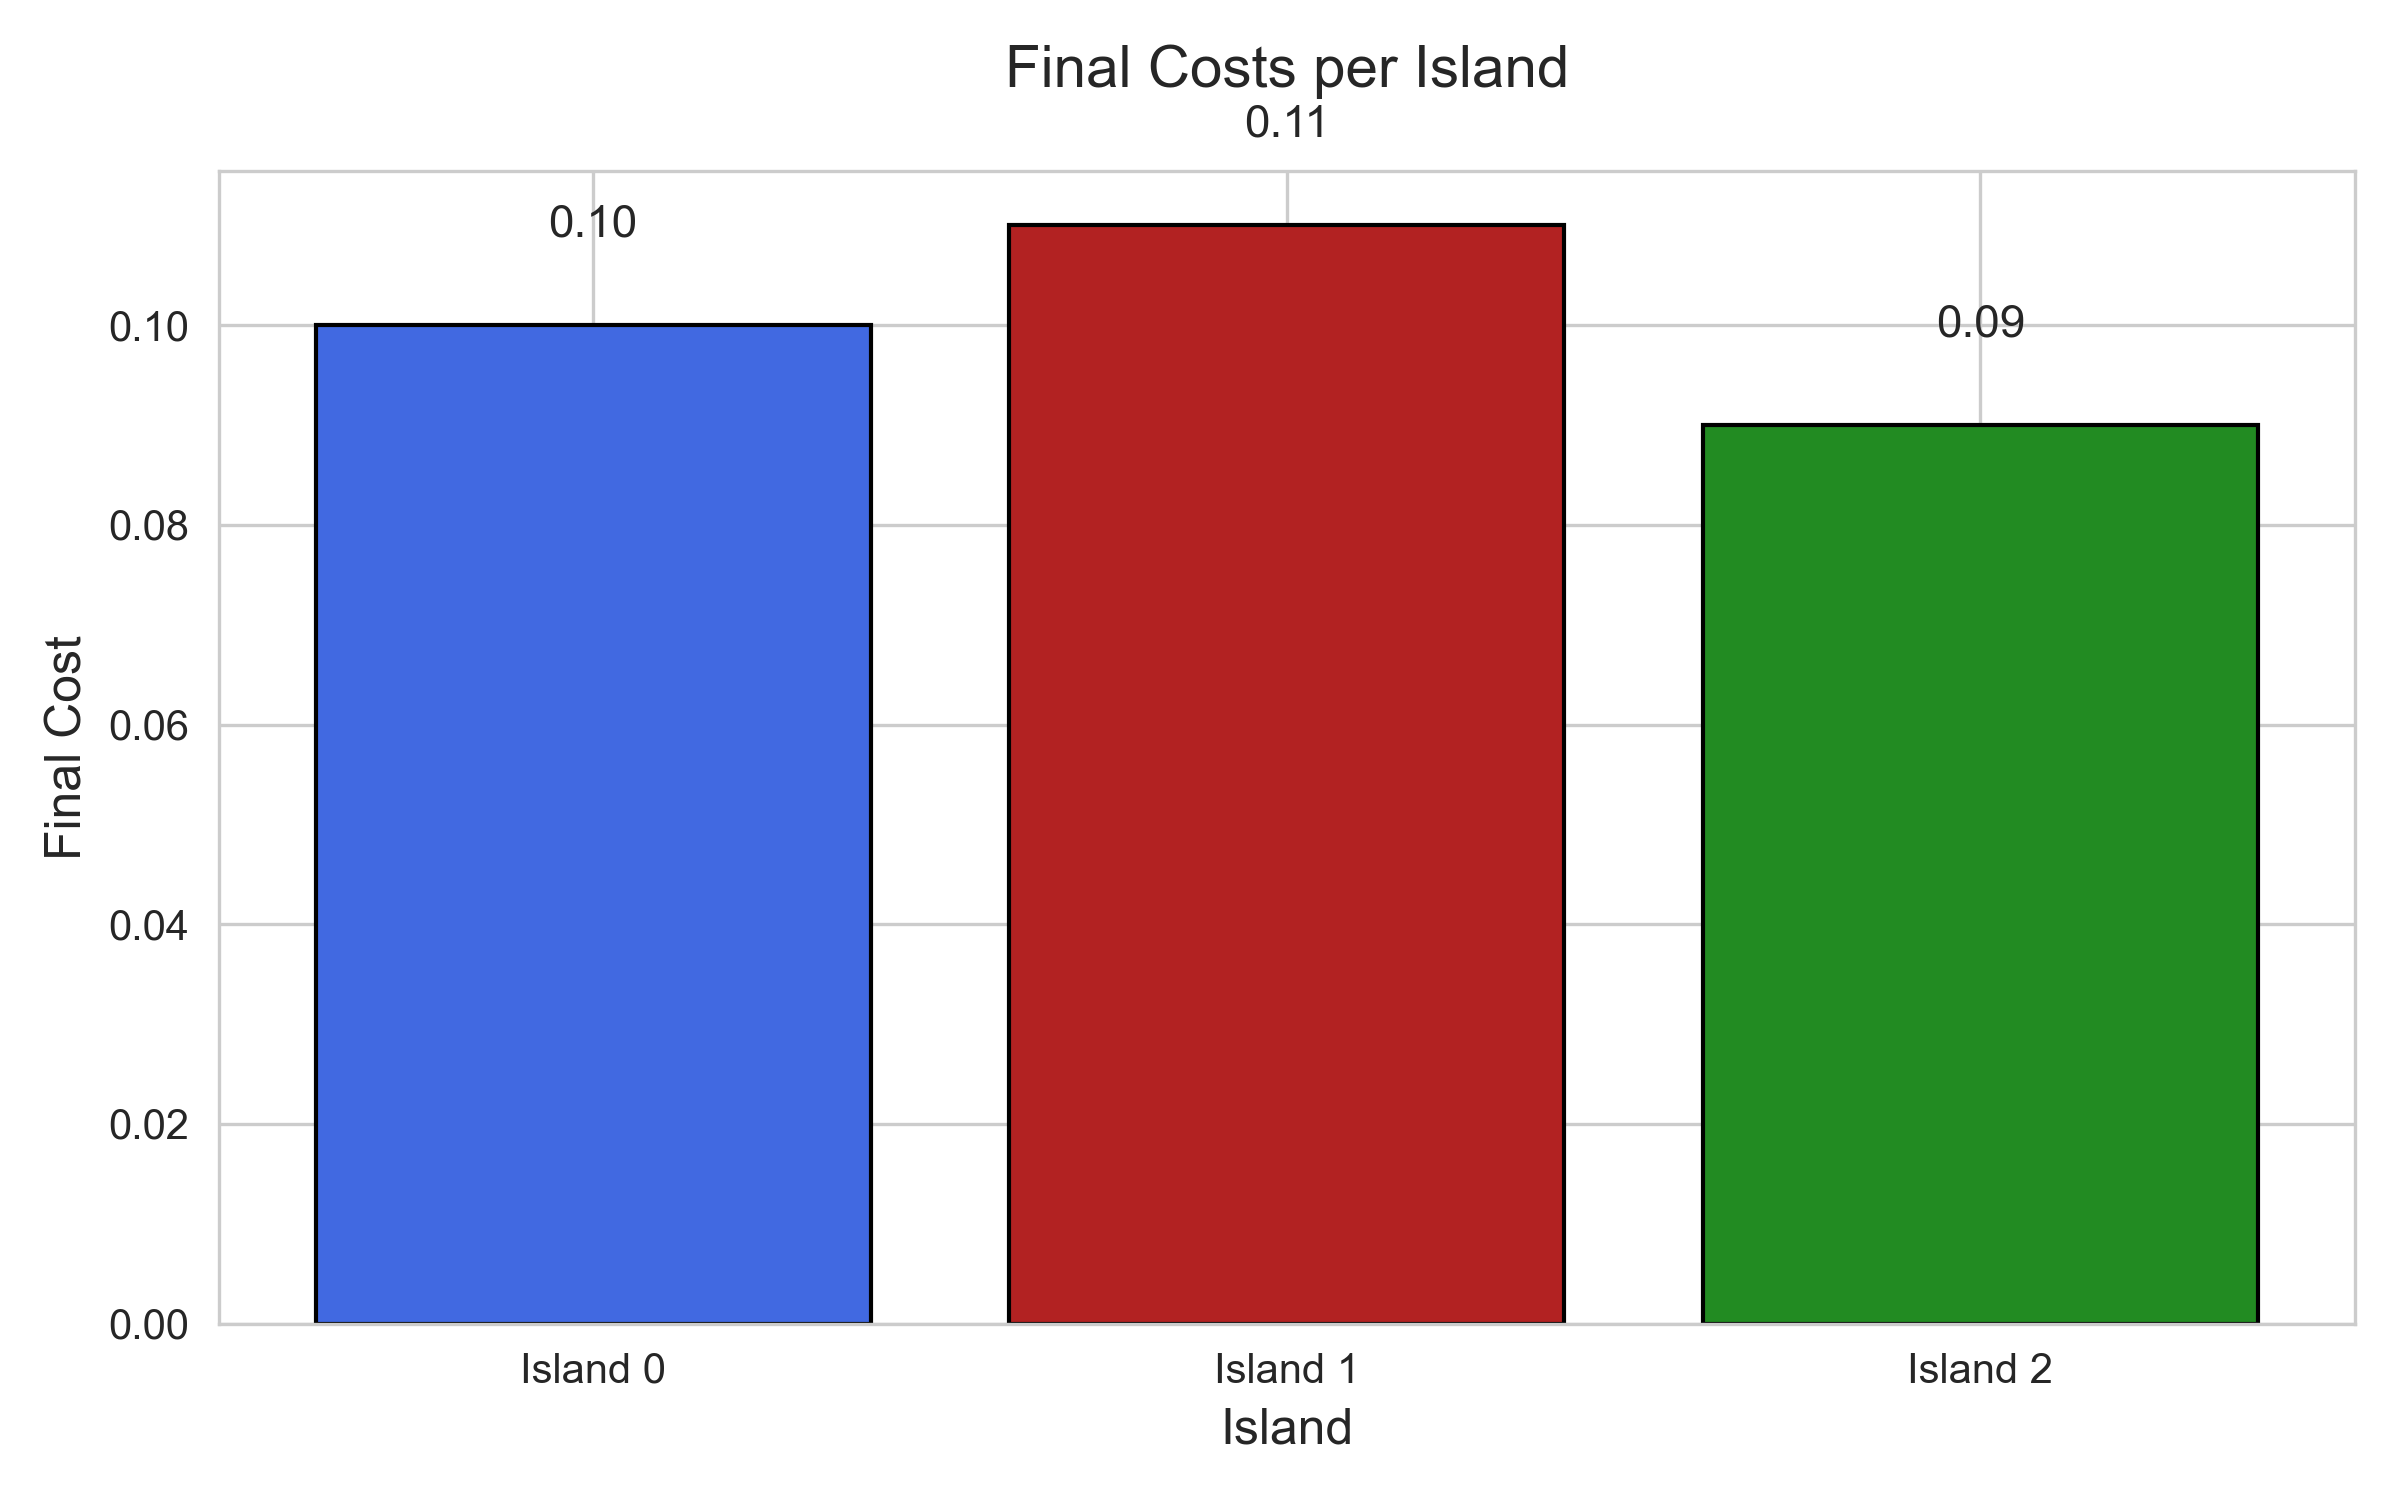
\includegraphics[width=0.75\textwidth]{img/final_costs_per_island.png}
    \caption{Distribuzione dei costi finali raggiunti da ciascuna isola.}
    \label{fig:final_costs_hist}
\end{figure}

\subsection*{Addestramento e valutazione del modello ottimizzato}

L'addestramento del modello LSTM con i migliori iperparametri trovati è stato monitorato mediante la train loss, 
come mostrato in Figura~\ref{fig:train_loss}. 
La curva evidenzia una discesa regolare e priva di overfitting, a conferma della buona generalizzazione.

\begin{figure}[H]
    \centering
    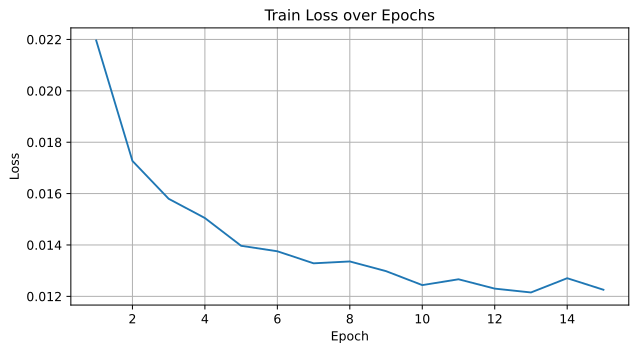
\includegraphics[width=0.8\textwidth]{img/Train Loss.png}
    \caption{Andamento della funzione di perdita durante la fase di addestramento del modello LSTM-CPSO.}
    \label{fig:train_loss}
\end{figure}

Le prestazioni finali del modello sono state valutate mediante metriche standard di regressione:

\vspace{0.5em}
\begin{itemize}
    \item \textbf{MAE} (Mean Absolute Error)
    \item \textbf{RMSE} (Root Mean Square Error)
    \item \textbf{$R^2$} (coefficiente di determinazione)
\end{itemize}
\vspace{0.5em}

\begin{table}[H]
    \centering
    \renewcommand{\arraystretch}{1.2}
    \begin{tabular}{lcccc}
        \toprule
        \textbf{Modello} & \textbf{Durata (s)} & \textbf{MAE} & \textbf{RMSE} & \boldmath$R^2$ \\
        \midrule
        LSTM - Island CPSO & 4\,200 & 0.03521 & 0.04598 & 0.9899 \\
        \bottomrule
    \end{tabular}
    \caption{Metriche di valutazione ottenute dal modello LSTM ottimizzato con algoritmo CPSO.}
    \label{tab:Result_LSTM_CPSO}
\end{table}

Infine, la Figura~\ref{fig:test_predict} mostra il confronto tra i valori predetti e quelli reali 
sul set di test. L’elevata corrispondenza tra le due curve testimonia la capacità del modello di 
generalizzare su sequenze temporali complesse.

\begin{figure}[H]
    \centering
    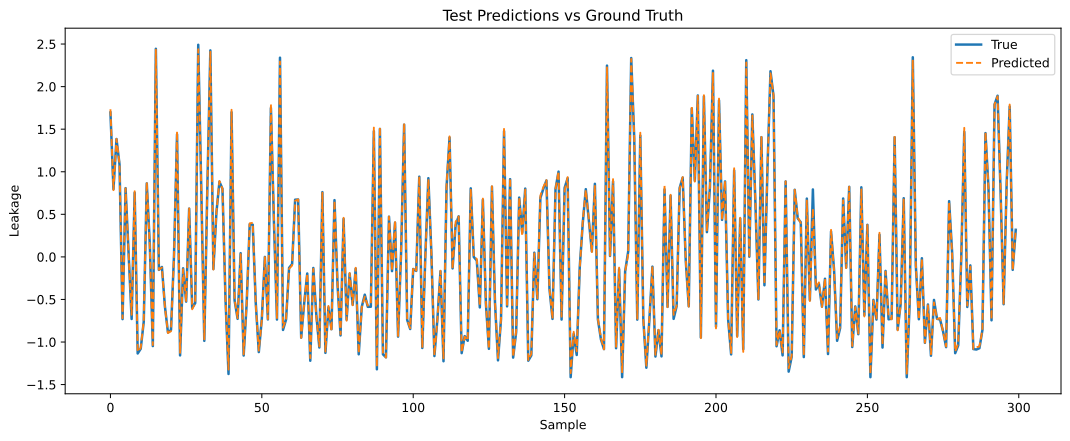
\includegraphics[width=0.8\textwidth]{img/Test Predict.png}
    \caption{Confronto tra valori reali e predetti nella fase di test del modello LSTM-CPSO.}
    \label{fig:test_predict}
\end{figure}

\section{Considerazioni Finali}

Nel complesso, i risultati ottenuti confermano l’efficacia dell’approccio CPSO a isole parallele nel fornire una 
strategia di ottimizzazione robusta ed efficiente per modelli di deep learning. L’integrazione tra ricerca continua, 
diversificazione delle soluzioni e sincronizzazione delle informazioni si è rivelata determinante nel raggiungimento 
di ottimi risultati predittivi.

In particolare, l’analisi grafica fornisce un importante supporto alla spiegabilità del processo di ottimizzazione: 
\begin{itemize}
    \item le curve di convergenza evidenziano l’evoluzione delle popolazioni locali;
    \item l’andamento del costo globale mostra l’impatto cumulativo della cooperazione tra isole;
    \item l’istogramma finale verifica la coerenza tra le soluzioni emerse.
\end{itemize}
Tali rappresentazioni facilitano l’interpretazione dei risultati anche in contesti applicativi critici, 
contribuendo alla trasparenza del modello.

L’integrazione tra un modello LSTM e un ottimizzatore CPSO si è dimostrata efficace nel catturare le 
dinamiche idriche complesse della rete simulata. L’approccio proposto consente di trasformare misure 
grezze eterogenee in una stima coerente e continua della perdita nel tempo, offrendo uno strumento utile 
per il monitoraggio predittivo e la gestione operativa delle reti idriche.

Inoltre, l’intera pipeline è pensata per essere generalizzabile: può essere facilmente estesa ad altri 
dataset, periodi temporali o configurazioni di rete, mantenendo inalterata la struttura metodologica. 
Questo rende il framework particolarmente adatto ad applicazioni pratiche in contesti reali, dove la 
flessibilità e l’adattabilità sono requisiti fondamentali.

Infine, i risultati ottenuti evidenziano come l’utilizzo di tecniche di ottimizzazione evolutiva possa 
migliorare sensibilmente le prestazioni di modelli di deep learning, riducendo al contempo la necessità 
di un’estesa fase di tuning manuale. Ciò apre interessanti prospettive future, sia in termini di 
automazione del processo modellistico, sia per l’integrazione con sistemi di decisione in tempo reale 
all’interno di infrastrutture intelligenti.

\bibliographystyle{ieeetr}
\bibliography{biblio}

\end{document}
